% --- Quantization ---
% ========== Part 3: Quantization ==========
\begin{frame}[plain]
  \centering
  \vfill
  {\LARGE\bfseries Quantization}
  \vfill
\end{frame}

% --- Part 3 narrative from Wang \& Spindler, NVIDIA Technical Blog (2025): model quantization concepts ---

\begin{frame}{Quantization}
  Quantization is a \textbf{key} compression technique for \textbf{LLMs} and \textbf{large transformers} to fit on \textbf{constrained hardware}. \newline
  \vspace{0.5em}
    \begin{itemize}\itemsep0.32em
      \item[\textcolor{red}{$\blacktriangleright$}] \textbf{Goal:} run larger models on \textbf{constrained} hardware with acceptable accuracy.
      \item[\textcolor{red}{$\blacktriangleright$}] Lowering precision on \textbf{weights and/or activations} (e.g.\ FP32/FP16 $\rightarrow$ FP8) cuts \textbf{memory}, speeds \textbf{inference}, and reduces \textbf{energy}---at some accuracy cost; the right trade-off is use-case dependent.
    \end{itemize}
\end{frame}

\begin{frame}{What to Quantize}
  \begin{itemize}\itemsep0.32em
    \item[\textcolor{red}{$\blacktriangleright$}] \textbf{Weights:} straightforward win on footprint; Llama~2 7B at FP16/BF16 $\approx$ \textbf{14\,GB} $\rightarrow$ FP8 weights $\approx$ \textbf{7\,GB} (blog numbers).
    \item[\textcolor{red}{$\blacktriangleright$}] \textbf{Activations:} intermediate layer outputs; quantizing compute can exploit \textbf{tensor cores} at lower bit width for more throughput.
    \item[\textcolor{red}{$\blacktriangleright$}] \textbf{KV cache} (decoder-only): grows with context, layers, and heads---often \textbf{several GB} at long context (e.g.\ 4096 tokens) alongside weights.
    \item[\textcolor{red}{$\blacktriangleright$}] \textbf{Deployment patterns:} weight-only INT8/INT4 for maximum weight memory savings (activations may stay higher precision); \textbf{KV cache quantization} when long context dominates.
  \end{itemize}
\end{frame}

\begin{frame}{Quantization Data Types}
  \begin{columns}[T,onlytextwidth]
    \column{0.46\textwidth}
    \begin{itemize}\footnotesize
      \item[\textcolor{red}{$\blacktriangleright$}] Floating point formats use their bits to store three parts: \textbf{sign} (positive/negative), \textbf{exponent} (size/range), and \textbf{mantissa} (precision of the value). For example, FP8 E4M3 uses 4 bits for the exponent and 3 bits for the mantissa.
      \item[\textcolor{red}{$\blacktriangleright$}] These numbers are represented as $x = (-1)^{\mathrm{sign}} \cdot 2^{\mathrm{exponent}} \cdot \mathrm{mantissa}$.
      \item[\textcolor{red}{$\blacktriangleright$}] Typical formats: FP32, FP16, BF16, FP8, and FP4. Main difference is how much range and precision you get—higher precision means more accurate numbers, but also more memory and compute. 
    \end{itemize}
    \column{0.52\textwidth}
    \centering
    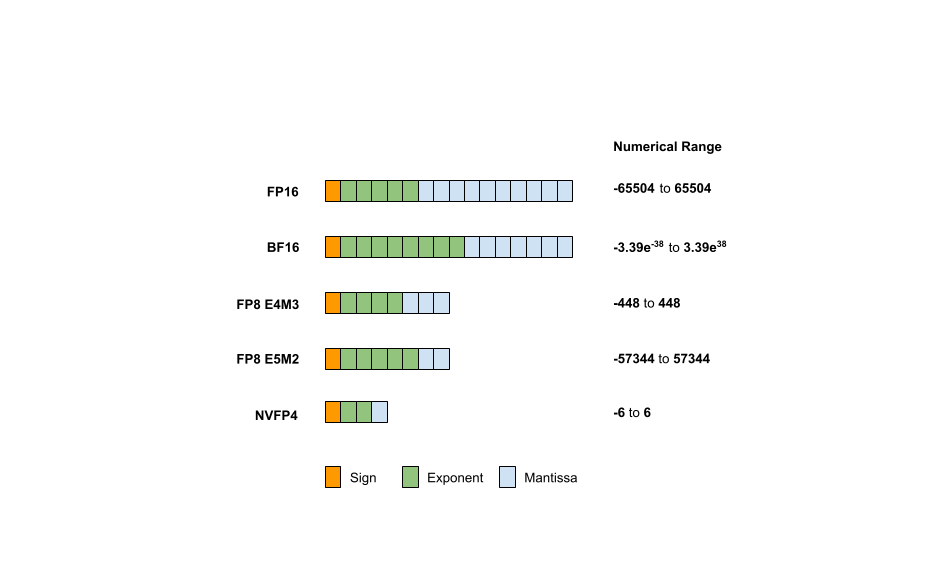
\includegraphics[width=\linewidth,height=0.78\textheight,keepaspectratio]{assets/New-Lecture-Inference_Optimisation/nvidia_blog_quant_fig1_fp_formats.png}\\[-0.2em]
    {\scriptsize Figure: FP16, BF16, FP8, FP4 layouts.}
  \end{columns}
\end{frame}

\begin{frame}{Quantization Granularity}
  \begin{columns}[T,onlytextwidth]
    \column{0.42\textwidth}
    \begin{itemize}\footnotesize
      \item[\textcolor{red}{$\blacktriangleright$}] \textbf{Per-tensor / per-layer:} one $(s,z)$ for the whole tensor---simplest, smallest metadata, can mis-handle heterogeneous ranges.
      \item[\textcolor{red}{$\blacktriangleright$}] \textbf{Per-channel:} separate parameters per channel (e.g.\ conv channels)---isolates \textbf{outliers} to their channel.
      \item[\textcolor{red}{$\blacktriangleright$}] \textbf{Per-block / per-group:} parameters per sub-block---finer control when mass varies inside a tensor.
    \end{itemize}
    \column{0.56\textwidth}
    \centering
    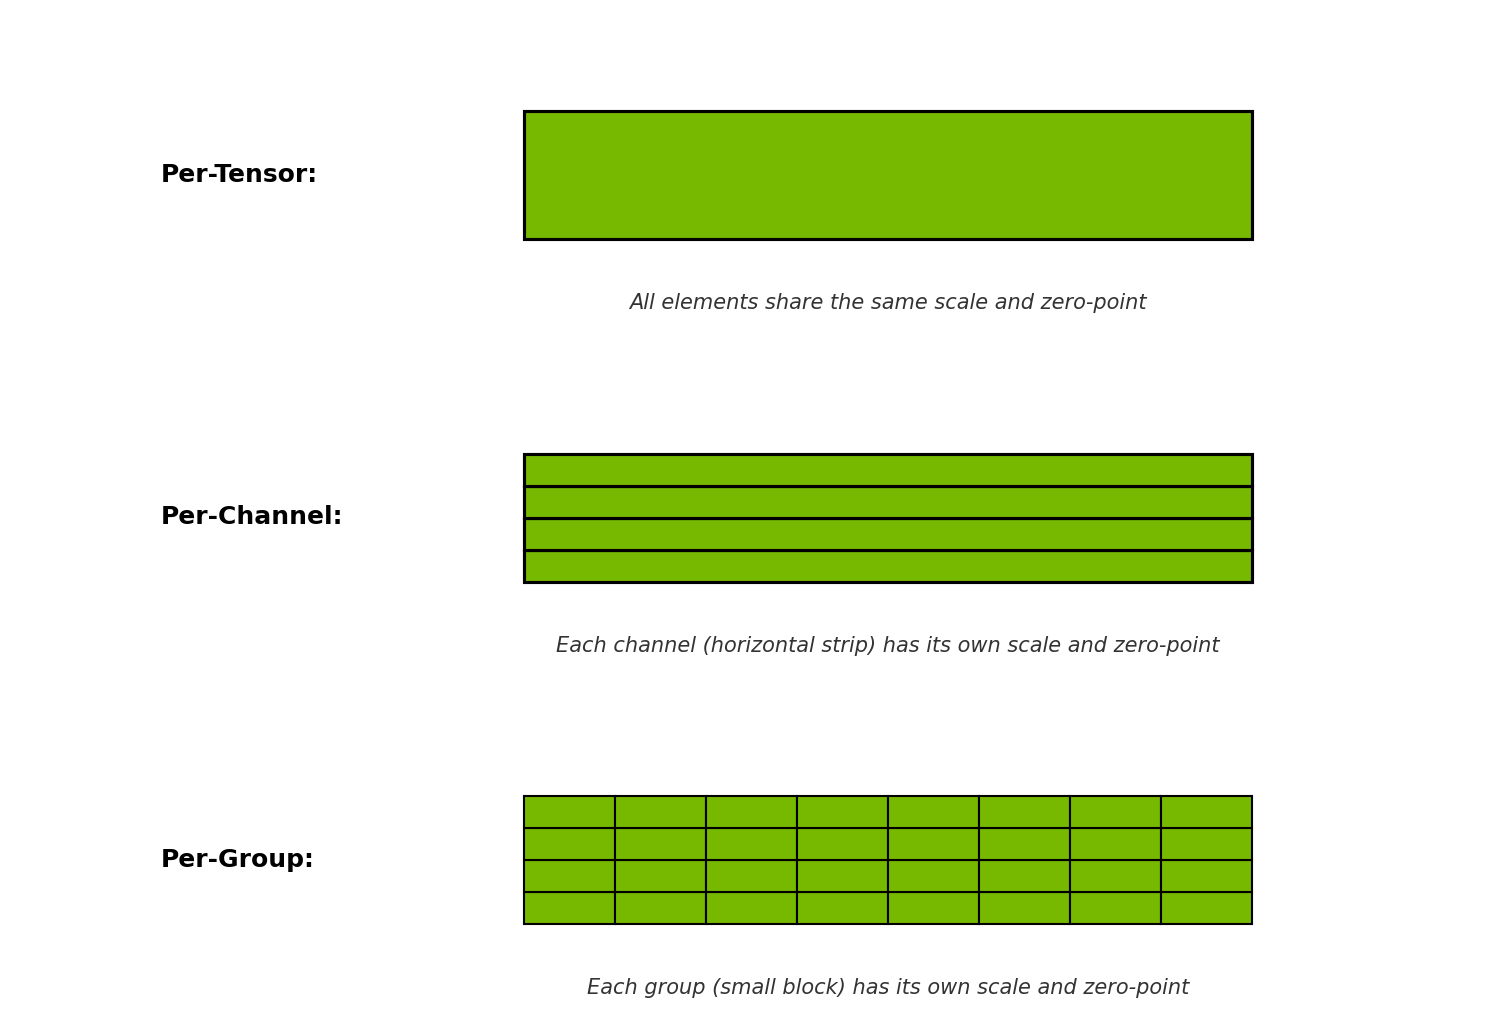
\includegraphics[width=\linewidth,height=0.8\textheight,keepaspectratio]{assets/New-Lecture-Inference_Optimisation/nvidia_blog_quant_fig4_granularity.png}\\[-0.2em]
    {\scriptsize Figure: per-tensor, per-channel, per-block.}
  \end{columns}
\end{frame}

% \begin{frame}{Affine vs.\ Symmetric Quantization}
%   \begin{columns}[T,onlytextwidth]
%     \column{0.44\textwidth}
%     \begin{itemize}\itemsep0.28em
%       \item[\textcolor{red}{$\blacktriangleright$}] Map $x \in [\alpha,\beta]$ to quantized $x_q \in [\alpha_q,\beta_q]$ using \textbf{scale} $s$ and (for affine) \textbf{zero-point} $z$ so real zero maps exactly---useful with zero-padded ops.
%       \item[\textcolor{red}{$\blacktriangleright$}] \textbf{Symmetric:} $z{=}0$; simpler and fewer adds; \textbf{TensorRT} and \textbf{Model Optimizer} focus on symmetric schemes in practice.
%       \item[\textcolor{red}{$\blacktriangleright$}] Rounding and \textbf{clipping} introduce error in both directions (quantize / dequantize).
%     \end{itemize}
%     \column{0.54\textwidth}
%     \centering
%     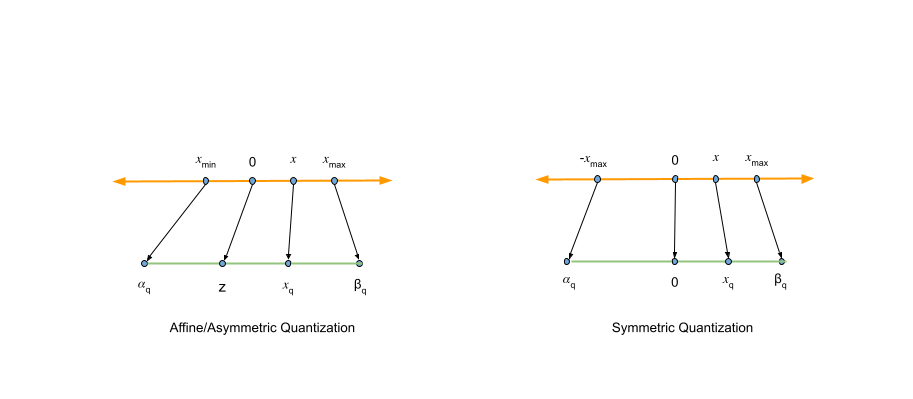
\includegraphics[width=\linewidth,height=0.78\textheight,keepaspectratio]{assets/New-Lecture-Inference_Optimisation/nvidia_blog_quant_fig2_affine_symmetric.png}\\[-0.2em]
%     {\scriptsize Figure~2: affine vs.\ symmetric (same blog).}
%   \end{columns}
% \end{frame}

\begin{frame}{Quantization-Aware Training (QAT)}
  \begin{itemize}\itemsep0.32em
    \item[\textcolor{red}{$\blacktriangleright$}] Bake quantization into training: forward/backward see \textbf{fake-quant} (quantize then dequantize) while master weights stay high precision for optimiser steps.
    \item[\textcolor{red}{$\blacktriangleright$}] Weights adapt to \textbf{rounding/clipping} error; fake-quant modules often \textbf{frozen} while weights are fine-tuned.
  \end{itemize}
\end{frame}

  % Two main approaches to post-training quantization (PTQ):

\begin{frame}{PTQ: Weight-Only and Weight+Activation Quantization (Overview)}
  \begin{itemize}\itemsep0.32em
    \item[\textcolor{red}{$\blacktriangleright$}] \textbf{Weight-only quantization:}
      Quantize the model's trained weights to lower precision using a calculated scale (with or without a zero-point). Since weights are fixed after training, no input data is needed.
    \item[\textcolor{red}{$\blacktriangleright$}] \textbf{Weights and activations quantization:}
      Requires representative input data to measure activation statistics (by running the model), which are then used to determine quantization parameters (scale and zero-point) through a process called calibration.
  \end{itemize}
\end{frame}

\begin{frame}{PTQ: Static vs.\ Dynamic Quantization}
  \begin{itemize}\itemsep0.32em
    \item[\textcolor{red}{$\blacktriangleright$}] \textbf{Static quantization:} 
    Calibration uses a dataset to determine quantization parameters once; these are kept fixed for all future inference.
    \item[\textcolor{red}{$\blacktriangleright$}] \textbf{Dynamic quantization:} 
    Quantization parameters are computed on the fly during inference for each input, so no calibration set is needed but more runtime overhead is incurred.
  \end{itemize}
\end{frame}

